\documentclass[border=0mm]{standalone}

\usepackage{import}
\subimport{../../../}{preamble.tex}

\usepackage{rotating}

\usepackage{tikz}
\usetikzlibrary{calc}
\usepackage{pgfplots}

\tikzset{
  partial ellipse/.style args={#1:#2:#3}{
    insert path={+ (#1:#3) arc (#1:#2:#3)}
  }
}

\begin{document}

\begin{turn}{-90}

  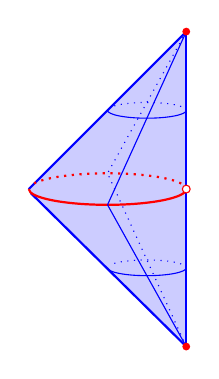
\begin{tikzpicture}[scale=0.5]

    \fill[blue!20] (2, 4) -- (2, -4) -- (-1.95, -0.1) -- (-2, 0) -- cycle;

    \draw[thick, blue] (2, 4) -- (2, -4);
    \draw[thick, blue] (2, 4) -- (-2, 0);
    \draw[thick, blue] (2, -4) -- (-1.95, -0.1);

    \draw[thick, red, dotted] (0,0) [partial ellipse=0:160:2cm and 0.4cm];
    
    \draw[thick, red] (0,0) [partial ellipse=180:360:2cm and 0.4cm];
    
    \draw[blue, dotted] (1,2) [partial ellipse=0:160:1cm and 0.2cm];
    \draw[blue] (1,2) [partial ellipse=180:360:1cm and 0.2cm];
    
    \draw[blue, dotted] (1,-2) [partial ellipse=0:160:1cm and 0.2cm];
    \draw[blue] (1,-2) [partial ellipse=180:360:1cm and 0.2cm];
    
    \draw[blue] (2, 4) -- (0, -0.4);
    \draw[blue, dotted] (2, 4) -- (0, 0.4);
    
    \draw[blue] (2, -4) -- (0, -0.4);
    \draw[blue, dotted] (2, -4) -- (0, 0.4);
    
    \node[circle, draw=red, fill=white, inner sep=1] at (2, 0) {};
    \node[circle, fill=red, inner sep=1] at (2, 4) {};
    \node[circle, fill=red, inner sep=1] at (2, -4) {};
  \end{tikzpicture}
\end{turn}
\end{document}

%%% Local Variables:
%%% mode: latex
%%% TeX-master: t
%%% End:
